\documentclass{article}
\usepackage[utf8]{inputenc}
\usepackage{hyperref}

\title{Experimental results on Bike Sales dataset}
\author{}
\date{}

\usepackage{natbib}
\usepackage{graphicx}

\begin{document}
\maketitle

\section{Data}
Experiments were conducted on the bike rentals data set that was made available by Capital-Bikeshare, and enriched with weather data by Fanaee-T et al.\ \cite{bike}.
The input features are: number of days since measuring began (trend), unit circle coordinate representation of the date (cosyear, sinyear), temperature (temp), feeling temperature (atemp), windspeed (windspeed) and humidity (hum).

\section{Training}
A XGBoost model was trained on the input features to predict the number of bike sales (mean-centered) on a given day.
A 80\%-20\% train test split was used, and the model was trained for 100 episodes in which the RMSE reduced from 1445 to 23.
The model has a RMSE of 671 on the test set. \emph{I increased the number of episodes. Any particular reason why we were using only ten before?}

%\section{Causal Shapley values}
%\begin{figure}[ht!]
%\centering
%\includegraphics[width=\textwidth]{sina_plot.pdf}
%%\includegraphics[width=1\textwidth]{sinaplot.png}
%\caption{The causal Shapley values on the test set}
%\label{fig:sinaplot}
%\end{figure}
%
%\newpage

In \autoref{fig:trendplot} we can see that the bikes sales are higher during summer, and lower during winter.
There are more sales in the second year than in the first year.
\begin{figure}[h!]
	\centering
	\begin{minipage}{.49\linewidth}
		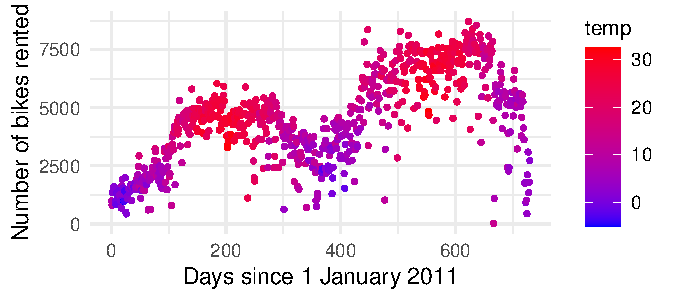
\includegraphics[width=\textwidth]{figures/trend_plot.pdf}
		%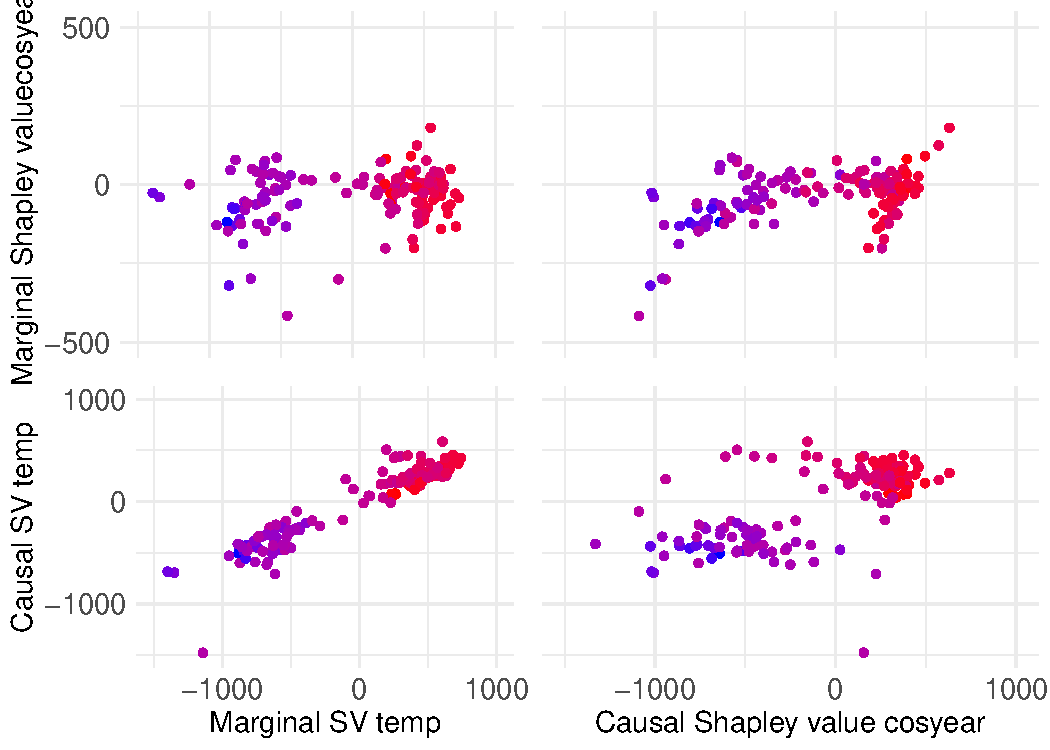
\includegraphics[width=\textwidth]{corr_plots.pdf}
		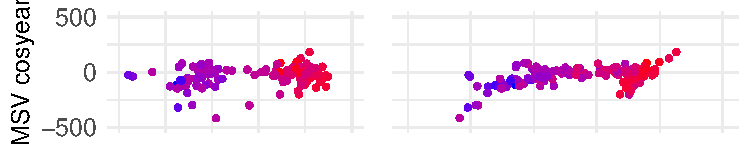
\includegraphics[width=\textwidth]{figures/corr_plots_top.pdf}
		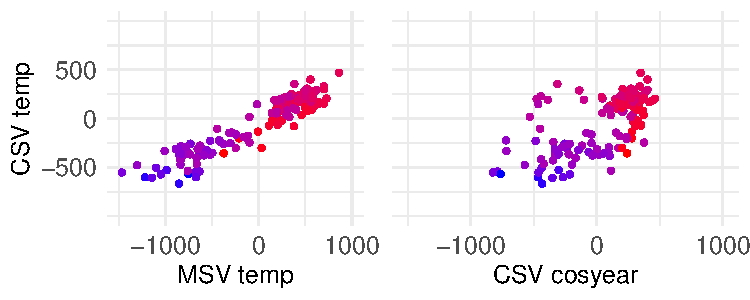
\includegraphics[width=\textwidth]{figures/corr_plots_bottom.pdf}
	\end{minipage}
	\begin{minipage}{.5\linewidth}
		\vfill
		\includegraphics[width=\textwidth]{figures/sina_plot.pdf}
	\end{minipage}
	\label{fig:trendplot}
	\caption{\textbf{top left}: Bike sales over time; \textbf{bottom left}: Correlation plots; \textbf{right}: Sina plot of causal Shapley values}
\end{figure}


In \autoref{fig:barplot} we can see the Shapley values for a single data point in winter.
The marginal approach attributes a lot to temperature (temp), while the causal approach attributes to both temperature and time of year (cosyear), which is congruent with \autoref{fig:trendplot}.

Not just for a single datapoint, but for the whole dataset we can see that the causal approach attributes to both season and temperature, shown in \autoref{fig:corrplot}.
Because they correctly integrate the causal structure of the input features, Causal Shapley values correctly explain why the model predicts higher bike sales on a cold summer day than on a warm winter day, even though they might have the same temperature.
README: I am not 100\% sure of this last sentence.

\begin{figure}[ht!]
\centering
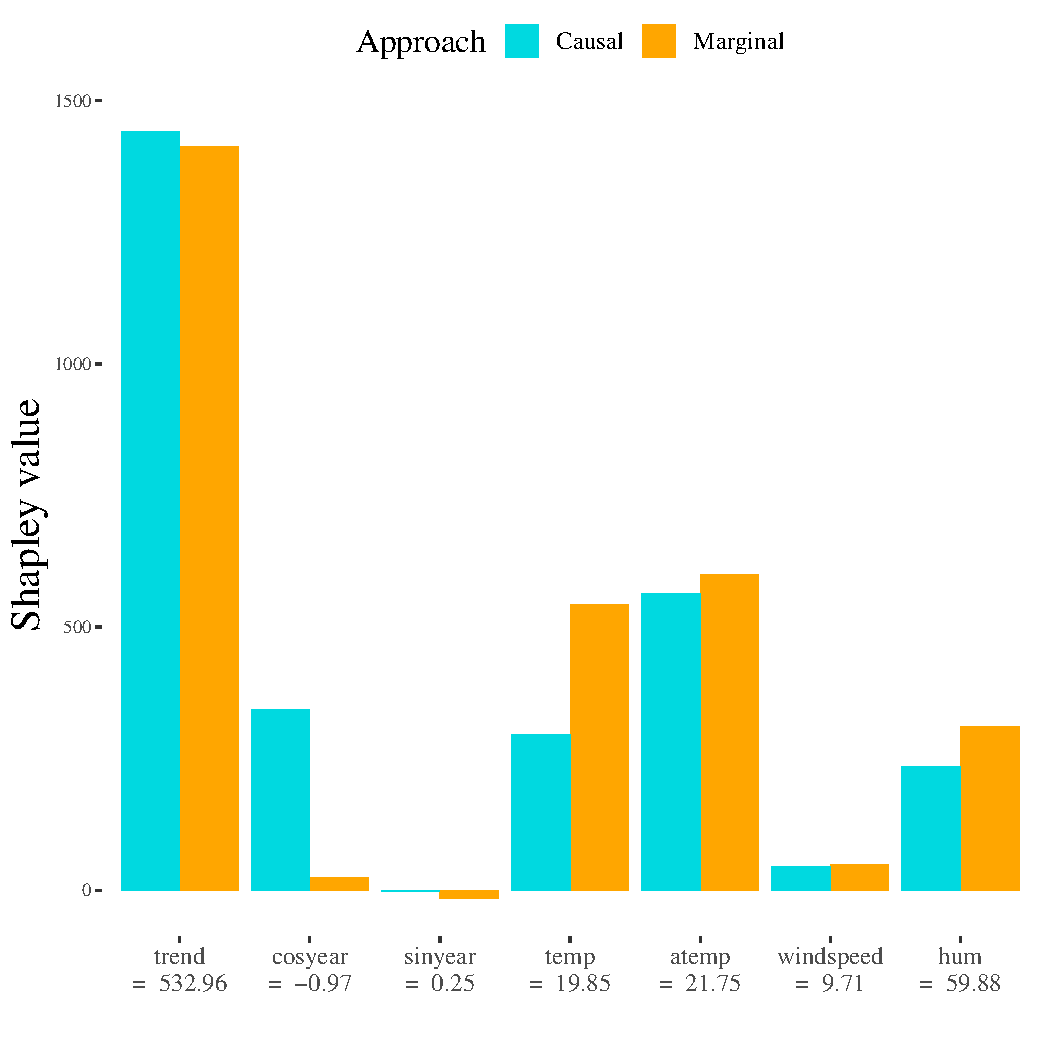
\includegraphics[width=1\textwidth]{figures/bar_plot.pdf}
% \includegraphics[width=1\textwidth]{barplot.png}
\caption{Causal and marginal Shapley values for a given data point}
\label{fig:barplot}
\end{figure}
\newpage



\bibliographystyle{plain}
\bibliography{references.bib}

\end{document}
